\documentclass[10pt,twoside,slovak,a4paper]{article}

\usepackage[slovak]{babel}
%\usepackage[T1]{fontenc}
\usepackage[IL2]{fontenc} % lepšia sadzba písmena Ľ než v T1
\usepackage[utf8]{inputenc}
\usepackage{graphicx}
\usepackage{url} % príkaz \url na formátovanie URL
\usepackage{hyperref} % odkazy v texte budú aktívne (pri niektorých triedach dokumentov spôsobuje posun textu)

\usepackage{cite}
%\usepackage{times}

\pagestyle{headings}

\title{Názov\thanks{Semestrálny projekt v predmete Metódy inžinierskej práce, ak. rok 2023/24, vedenie: Meno Priezvisko}} % meno a priezvisko vyučujúceho na cvičeniach
\title{Hĺbkova analýza dát a jej využitie v praxi}
\author{Patrik Török\\[2pt]
	{\small Slovenská technická univerzita v Bratislave}\\
	{\small Fakulta informatiky a informačných technológií}\\
	{\small \texttt{xtorok@stuba.sk}}
	}

\date{\small 5. november } % upravte



\begin{document}

\maketitle

\begin{abstract}
Vedomosti boli odjakživa dôležitou súčasťou ľudskej spoločnosti. Postupom času by sa bez pomoci technológie proces získavania poznatkov stal čoraz ťažším, pretože každým dňom narastá počet dát a údajov, ktoré treba pre nadobudnutie znalosti spracovať. Hĺbková analýza dát označuje proces alebo metódu, ktorá z veľkého množstva údajov získava zaujímavé poznatky. Tento proces možno aplikovať v rôznych oblastiach ľudského života vrátane podnikania, vzdelávania, sociálnych sietí, medicíny, vedy apod. Oblasť hĺbkovej analýzy má teda široké uplatnenie aj v oblasti vedeckého pokroku a porozumenia. Cieľom tohto článku je čitateľovi predstaviť proces hĺbkovej analýzy, stručne ho oboznámiť s evolúciou hĺbkovej analýzy údajov od prvej zmienky po súčasnosť a vymenovať konkrétne oblasti, v ktorých sa tento proces využíva, spolu s opisom využitia v spomenutej oblasti priemyslu. 
$$ \cdots $$
\end{abstract}



\section{Úvod}
Hĺbková analýza dát (angl. Data mining) je proces pri ktorom sa spracúva veľké množstvo informácií a následne sa premieňa na vedomosť\cite{Iberdola}. Je akousi kombináciou štatistiky a umelej inteligencie, vďaka čomu môžu spoločnosti vytvárať modely, ktoré im úmožnia nacházať súvislosti medzi miliónmi záznamov. Zároveň vďaka tomuto procesu dokážu spoločnosti predpovedať trendy budúcnosti. Keďže množstvo informácií, ktoré treba spracovať, neustále rastie,  hĺbková analýza dát nachádza čoraz väčšie uplatnenie v mnohých priemyselných oblastiach. Množstvo spoločností používa softvér na hĺbkovú analýzu údajov, vďaka ktorému sa môžu dozvedieť viac o svojich zákazníkoch. Programy na hĺbkovú analýzu totiž hľadajú súvislosti v údajoch na základe informácií, ktoré používatelia od programu vyžadujú alebo programu poskytujú. Tiež im môže im pomôcť v reklamnej oblasti, napr. pri vytváraní efektívnejších marketingových stratégií, zvyšovaní predaja a znižovaní nákladov.\cite{Bidgoli:HTM} Hĺbková analýzy sa opiera o efektívne zhromažďovanie, uskladnenie a spracovanie údajov. Jej vplyv je citeľný aj mimo technickej sféry, s jej rozšírením vzrástli obavy o súkromie dát a bezpečnosť. Preto došlo k zavedeniu mnohých regulácií, ako napríklad GDPR, a začal byť kladený väčší dôraz na dodržiavanie zodpovedný a etických postuov tohto procesu.
\section{Typy hĺbkovej analýzy dát}
Aby dosiahli požadovaný výsledok, dátoví vedci a analytici používajú rôzne typy hĺbkovej analýzy údajov. Medzi najbežnejšie techniky patria:
\begin{itemize}
\item Zhluková analýza (eng. Clustering)\\
Zhlukova analýza je v podstate hľadanie skupín s podobnými vlastnosťami. Obchodníci, a zamestnanci v oblasti reklamy často používajú tento typ hĺbkovej analýzy na to, aby identifikovali cieľové skupny. Zhlukova analýza je užitočná vtedy, keď spoločnosti nevedia, aké podobnosti by mohli existovať v rámci ich uložených údajov.
\item Detekcia anomálií\\
Tento typ hĺbkovej analýzy vyhľadáva vyčnievajúce dáta v dátovom súbore, čo môže pomôcť pri odhaľovaní podvodov.
\item Regresia\\
Regresia patrí medzi pokročilejšie štatistické nástroje. Používa sa najmä v prediktívnej analýze, využívajú ju hlavne vývojári, ktorí hľadajú spôsoby, ako zvýšiť počet použivateľov, a pomáha predpovedať budúce výnosy s minimálnym rizikom.
\item Dolovanie z textu\\
Dolovanie z textu analyzuje, ako často ľudia používajú určité slová. Môže byť použitá na zistenie nálady autora textu alebo osobnosti, ako aj na analýzu príspevkov na sociálnych sietiach na marketingové účely alebo na odhalenie potenciálnych únikov údajov od zamestnancov.\cite{EmmaCroc}

\end{itemize}

\section{Proces hĺbkovej analýzy dát} 
Dátoví analytici v procese hĺbkovej analýzy údajov často pracujú podľa určitého postupu krokov. Ak by postupovali inak, existuje možnosť, že sa pri analýze dostanú do problémov. Počet krokov pre typy hĺbkovej analýzy sa môže líšiť, no všetky postupnosti krokov sú odvodené od všeobecnej postupnosti, ktorá vyzerá takto:\\
\begin{itemize}
\item Krok 1: Musíme zistiť, čo chceme hĺbkovou analýzou dosiahnuť, aké ciele naplniť a zistiť, ako ukončiť proces s úspechom. Následne treba uvažovať o tom, aké zdroje sú k dispozícii, ako budú zabezpečené a uložené, ako bude prebiehať zhromažďovanie informácii a ako bude vyzerať konečný výsledok alebo analýza. Tento krok zahŕňa aj stanovenie obmedzení údajov, ich ukladania, zabezpečenia a zberu a posúdenie vplyvu týchto obmedzení. \\
\item Krok 2: Až potom začneme pracovať so samotnými dátami. Môžeme ich zhromažďovať, nahrávať a extrahovať. Potom sa vyčistia od odchýlok a skontrolujú sa, chybné a neopodstatnené dáta sa odstránia. Môže sa skontrolovať aj veľkosť objemu dát, pretože čím väčší je súbor informácií, tým viac zabere analýza času. \\
\item Krok 3: Po získaní čistého súboru údajov môžeme začať s hľadaním vzťahov, trendov, asociácií alebo sekvenčných vzorcov. Údaje tiež môžme načítať do prediktívnych modelov, vďaka ktorým môžeme predpovedať trendy budúcnosti. \\
\item Krok 4: Po ich získaní možno výsledky sumarizovať, interpretovať a prezentovať nadriadeným, ktorí doteraz do procesu hĺbkovej analýzy neboli zapojení a tí môžu na základe spomínaných výsledkov vykonať plánovaný krok spoločnosti alebo zmeniť svoje rozhodnutia.\\
\item Krok 5:Manažment spoločnosti reaguje na zistenia, a na ich základe príjme opatrenia. Ak sa spoločnosť rozhodne, že zistenia analýzy neboli  presvedčivé, môže požadovať zopakovanie procesu. Ak sú zistenia dostatočne presvedčivé, môže spoločnosť na ich základe obrátiť pozornosť podľa výsledku analýzy.\cite{CraigSTD}\cite{IBM}\\
\\
\end{itemize}
\begin{figure}
    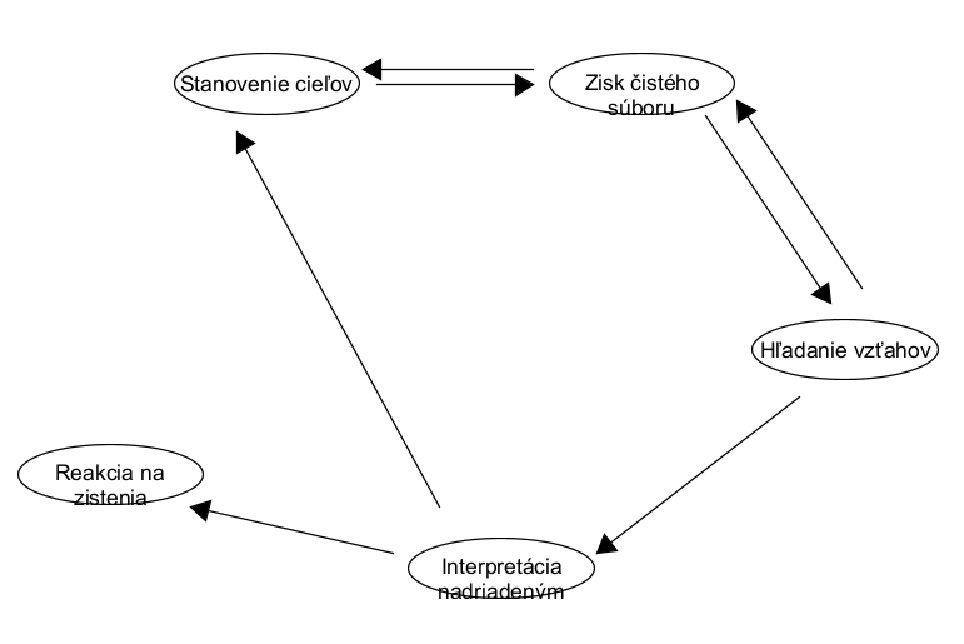
\includegraphics[width=1\linewidth]{diagram datamining.pdf}
    \caption{Enter Caption}
\end{figure}

\section{História}
História hĺbkovej analýzy dát je dôkazom rýchlosti vývoja analýzy dát a jej stále väčšej dôležitosti v rôznych oblastiach. Počas vývoja prešla niekoľkými kľúčovými fázami.

\subsection{Začiatky (60-80-te roky 20. stor.)} 
Počiatky hĺbkovej analýzy siahajú do 60-tych a 70-tych rokov 20. stor., keď štatistici a výskumníci prvýkrát začali preskúmavať metódy na analýzu dát.
Počas tohto obdobia sa vyvinuli základné techniky, ako je analýza zhlukov a algoritmy stromu rozhodnutí. Tieto metódy položili základy pre ďalší vývoj hĺbkovej analýzy.

\subsection{Zrodenie hĺbkovej analýzy (90-te roky 20. stor.)} 
90-te roky predstavujú vytvorenie moderných spôsobov hĺbkovej analýzy, vznikol samotný pojem "Hĺbková analýza dát". Pokrok v oblasti výpočtovej techniky a rozšírenie databáz umožnili vznik tohoto procesu ako samostatného odboru. Výskumníci a praktici začali vyvíjať špeciálne algoritmy a nástroje na odhalenie cenných poznatkov v rozsiahlych súboroch dát. Preto boli v tomto období vyvinuté kľúčové koncepty a techniky, ktoré dodnes tvoria jadro hĺbkovej analýzy.

\subsection{Rozšírené použitie (začiatok 21. storočia)} 
Na začiatku 21. storočia sa hĺbková analýza dát stala dostupnejšou. Mnohé organizácie spoznali jej potenciál pre získavanie poznatkov z dát, a vyvinuli softvérové nástroje, ktoré tento proces zjednodušovali. Rozvoj digitálnych dát, sociálnych sietí a internetu priviedla k vzniku "big data", ktoré prinieslo nové výzvy a príležitosti pre ťažbu dát. Počas tohoto obdobia boli vyvinuté mnohé technológie na spracovanie veľkého množstva dát.
\subsection{Strojové učenie (2010 - súčasnosť)}
Po roku 2010 sa hĺbková analýza zlúčila so strojovým učením, keďže sa algoritmy strojového učenia stali dôležitými pre urýchlenie analýzy dát. Pokroky výpočtovej techniky a rozsiahle dátové úložiská umožnili presnejšie a komplexnejšie vykonať proces hĺbkovej analýzy.
\\
\\
V súčasnosti zostáva proces hĺbkovej analýzy neoddeliteľnou súčasťou dátovej vedy. Dátoví vedci využívajú sofistikované algoritmy a nástroje na získavanie cenných poznatkov z dát, čím pomáhajú podnikom pri dôležitých rozhodnutiach. Čo sa budúcnosti týka, očakáva sa, že hĺbková analýza bude pokračovať v rozvoji, aby spĺňala požiadavky sveta stále bohatšieho bohatého na dáta, bude zohrávať kľúčovú úlohu pri rozvoji umelej inteligencie a modelov strojového učenia, aby organizácie mohli naďalej získavať zmysluplné informácie z rastúceho objemu dát.\cite{Majid:Evolution}

\section{Výhody a nevýhody}
Výhody a nevýhody hĺbkovej analýzy možno vidieť v nasledujúcej tabulke:

\begin{table}[h!]
    \centering
    \begin{tabular}{|c||c|}
        \hline
         Výhody &  Nevýhody\\
         \hline\hline
         Efektivita & Komplexnosť\\
         \hline
         Všestrannosť & Vysoké náklady\\
         \hline
         Odokrýva skryté informácie & Neistota úspechu\\
         \hline
    \end{tabular}
    \caption{Výhody a nevýhody hĺbkovej analýzy dát\cite{AlexandraTwin}}
    \label{tab:my_label}
\end{table}
\subsection{Výhody}
\begin{itemize}
\item Hĺbková analýza dát zabezpečuje, že spoločnosť zhromažďuje a analyzuje spoľahlivé údaje. Často ide o prísnejší, štruktúrovaný proces, ktorý formálne identifikuje problém, zbiera údaje ktoré súvisia s daným problémom a snaží sa nájsť riešenie.\cite{LunaCamp}
\item Hĺbková analýza dát môže na prvý pohľad vyzerať v rôznych aplikáciách veľmi odlišne, ale celkový proces sa dá použiť takmer v každej novej alebo staršej aplikácii. V podstate je možné zhromažďovať a analyzovať akýkoľvek typ údajov a takmer každý problém je možné riešiť pomocou hĺbkovej analýzy.
\item Cieľom hĺbkovej analýzy je vziať nespracované informácie a určiť, či medzi údajmi existuje nejaká súvislosť. To umožňuje spoločnosti hodnotne narábať s  informáciami, ktoré má k dispozícii a ktoré by sa na prvý pohľad nedalo postrehnúť. Dátové modely sú často zložité, no odhaľujú skryté trendy, vďaka ktorým sa môžu spoločnosti prispôsobiť a navrhnúť obchodné stratégie.\cite{AlexandraTwin}
\end{itemize}
\subsection{Nevýhody}
\begin{itemize}
\item Náročnosť procesu hĺbkovej analýzy je jednou z jej najväčších nevýhod. Od dátových analytikov sa očakávajú určité technické zručnosti a schopnosť pracovať s daným softvérom. 
\item Hĺbková analýza negarantuje, že jej výsledok prinesie spoločnosti zisky. Môže sa vykonať štatistická analýza, na základe získaných dát sa môžu prijať opatrenia, no spoločnosti z nich nemusia vždy benefitovať. To môže byť spôsobené dôsledkom nepresných zistení, neočakávaných zmien na trhu alebo chybami samotného modelu.
\item Získavanie údajov pomocou hĺbkovej analýzy je spojené aj s vysokými nákladmi. Dátové nástroje často nie sú voľne dostupné, vyžadujú vysoké predplatné a získanie niektorých častí údajov je nákladné.\cite{AlexandraTwin}
\end{itemize}


\section{Aplikácie a využitie v praxi}




\bibliography{literatura}
\bibliographystyle{plain} % prípadne alpha, abbrv alebo hociktorý iný
\end{document}
